\chapter{Literature Survey}
Literature survey is split in three parts, (i) design and development of PMU, (ii) Computation of phasor estimate and (iii) testing procedures for standard compliant testing.


\section{PMU architecture}
A survey was made of the PMUs designed developed elsewhere in the academia for knowing the experience, best practices and targeted performance and ways of implementation. Few PMU implementation worth noting here are as follows:

\subsubsection{GRIDTrak PMU} It is one of the oldest synchrophasor implementation, a PMU developed by University of Baltimore \cite{dotta2014teaching} was aimed towards teaching measurement of AC synchrophasors' frequency, amplitude and angle. It used set of Op-amp and voltage comparators to convert input sine to square and was using accurate timer to measure the distance between two zero crossings. An accurate timer was also keeping track of offset between 1PPS signal and the zero crossing for phase measurement, it was using an ideal sine wave of the input signal for measuring amplitude. Data is also transmitted based on the IEEE Std. C37.118-2005 specifications. The aim of the GridTrak device is to produce a PMU that is not costly and one that can be widely distributed among researches and amateur enthusiast \cite{stadlin2013gridtrak}.

\subsubsection{DTU- PMU}
This PMU implementation was developed at Denmark Technology University (DTU) during year 2005-2007 \cite{garcia2010dtu} and was one of the high-end implementation of that time. The DTU-PMU is made up of two PCs that work together to provide PMU functionality.
\begin{figure}
	\centering
	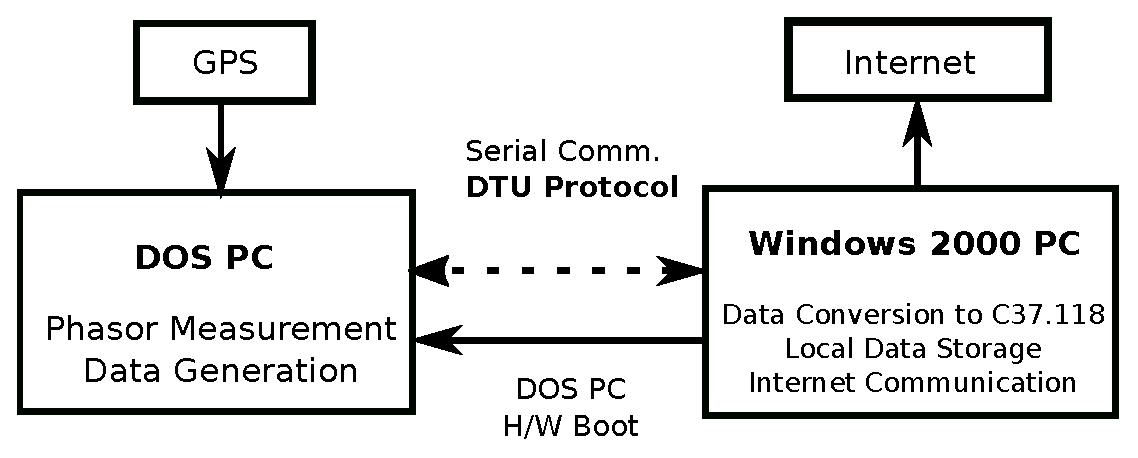
\includegraphics[scale=0.4]{fig/DTU-PMU.eps}
	\caption{DTU-PMU Implementation}
	\label{fig:dtu-pmu}
\end{figure}

 As show in Fig: \ref{fig:dtu-pmu} one of the PC acts as an data acquisition unit, which handles I/Os, GPS timing and UART peripherals, this system runs on a classic Disk Operating System (DOS). The second PC acts as an communication bridge, it frames the data received from the PC1 in C37.118.2 format, and send it to the PDC as well as stores it locally. This setup was not a low cost implementation due to which it makes its usage and implementation limited. This PMU implemented adaptive signal sampling which synchronizes the sampling done by the device with the input signal frequency. A 16-bit ADC was used to take in 64 or 128 samples/cycle.  A simple FFT was done to extract only the fundamental frequency component for estimating the phasor(s). GPS interface was ensuring accurate UTC synced time reference which was accurate up to   $ \pm 100$ ns, internal oscillator was ensuring that the sampled frame timestamp is in tight sync to the GPS dictated UTC time, via 1 PPS correction and NMEA time messages. 
 
 \subsubsection{OpenPMU}
 It is a PMU development project under active development at Queen's University, Belfast \cite{paper:openpmu} . This project intends to develop a competitive open source PMU device whose performance is compliant to the standards and is equally good as proprietary PMUs, designed and developed using IP protected algorithms. 
 
 \begin{figure}[h]
 	\centering
 	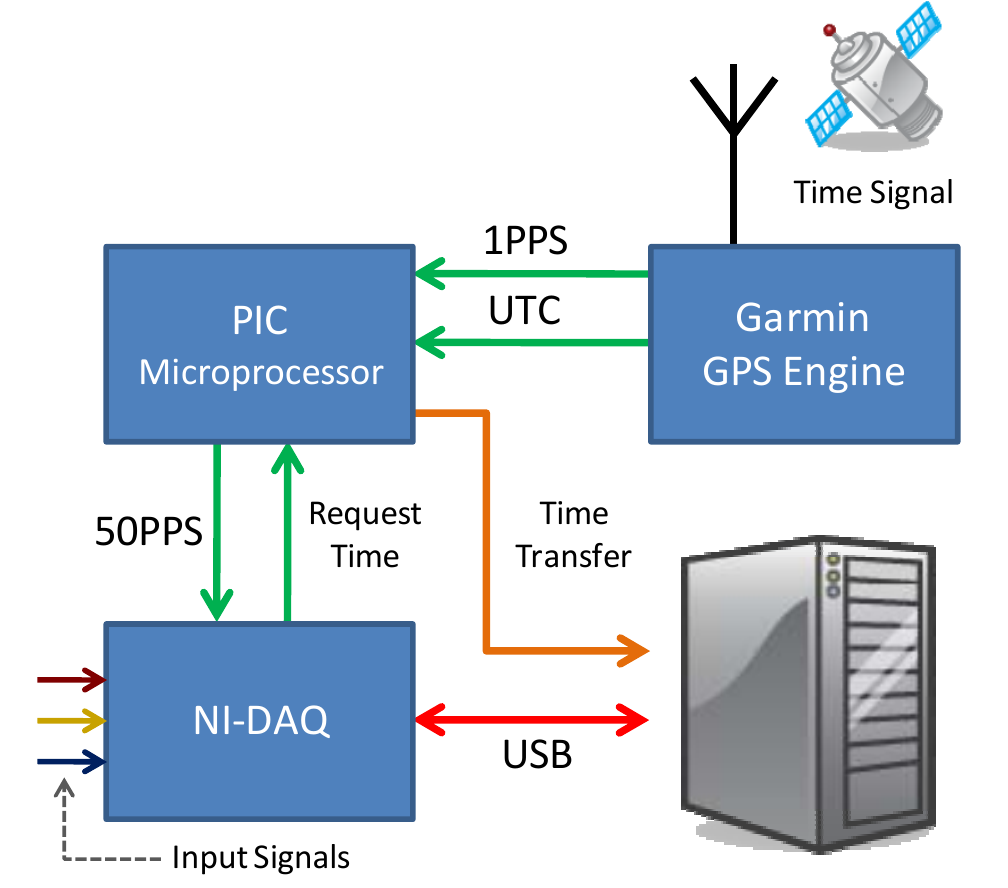
\includegraphics[scale=0.5]{fig/OpenPMU.png}
 	\caption{OpenPMU Architecture}
 	\label{fig:OpenPMU}
 \end{figure}    
 
 Fig: \ref{fig:OpenPMU} shows implementation of OpenPMU. Its design can be split into two parts measurement part (ADC sampling and GPS time) and analysis part. Measurement part uses National Instrument's a standard Data Acquisition device (DAQ) card and GPS module produced by Garmin. National Instruments  and Garmin are perhaps some of the most expensive manufacturers, which makes this design a very costly implementation right away. On the analysis side, standard x86/64 bit PC was used. The design policy was to keep both parts asynchronous allowing independent development of each of them.
 
 \subsubsection{Conclusion}
 From the literature survey it was quite clear that what criteria we should aim at for our implementation. Few points observed are as follows:
 \begin{itemize}
 	\item Low Cost: In case if DTU-PMU and OpenPMU the overall cost of device will go very high, due to very grandeur design using two computer, or NI's DAQ cards. So our implementation needs to be cost effective.
 	\item Reliability: All implementation aims to have a reliable system, (even at the higher cost) which if can be achieved at lower cast would be an achievement.
 	\item Ease of development: Hardware side design was quite simple due to use of proprietary devices on the analysis side, use of appropriate algorithm via a user friendly language for phasor estimation would be a big plus. DTU-PMU uses DOS bases system which is tough to code, or else in case of OpenPMU a .NET and C\# based design, which are framework requiring  expertise. Instead if, Python or equivalent language is used then it would be great value addition, as focus can be kept on logic rather then implementation.
 	\item Size: All of the above implementation are bulky, two PC based DTU-PMU, or PC based OpenPMU are not a very elegant setup. If size can be reduced and device can be made portable, that would be of great value.
 \end{itemize} 
 
 \section{Computation of Phasors}
 PMU algorithms is a research topic in itself. Precise phasor estimate plays a vital role in real-time operation of the device. PMU algorithms are evaluated and classified on the basis of their computation complexity or their domain of estimation (frequency or time). There are number of papers dealing with phasor computation from sampled data out of which they can be classified primarily in to two parts (i) Fourier Transform (DFT) based (ii) Non-DFT based method. Number of papers existing in literature deal with Fourier transform based method but there are other papers which deals with use of Least-square methods, Kalman filter Method, Prony methods, Newton type algorithm, Iterative DSP technique etc., are to name a few. Choosing a method is always a trade of between computational requirement, accuracy and complexity. For our PMU design, we needed a method which is computationally less intensive, fast and yet accurate. The recursive DFT method described in the paper \cite{phadke1983new}, which proposes that processing of progressive window can be optimized by retaining 2(N-1) multiplication and 2(N-1) summation of the data which is common between new and old data frame is worth mentioning here. A recursive computation of this type is made possible by the fact that DFT computation is arbitrary to the extent of it's phase angle \cite{phadke1983new}. As stated in the paper new value can be obtained from the old value using the following formula:
 
 \begin{equation}
 X_{re}^{(new)} = X_{re}^{old} + \frac{2}{N}cos 2\pi(x_{n} - x_{o})
 \label{eq:recurDFT1}
 \end{equation} 
 
 \begin{equation}
 X_{im}^{(new)} = X_{im}^{old} + \frac{2}{N}sin 2\pi(x_{n} - x_{o})
 \label{eq:recurDFT2}
 \end{equation}
 
 As show in equation \ref{eq:recurDFT1} \& \ref{eq:recurDFT2}, by reusing the previous values recursively computation can be reduced and there by computation time. This equations have been used for phasor computation in our PMU. Apart from recursive DFT there are several other methods were considered, like plain DFT and a mix-radix FFT \cite{kissFFT} along with blackman-harris windowing and Hamming window function. 
 
 For frequency computation, the exists several methods which includes but are not limited to DFT, recursive phasor phase change, least square technique. After evaluating several methods an iterative method described in \cite{sidhu1998iterative} was chosen, which is one of the simplest and widely used method for frequency computation. As described in the paper frequency can be computed from:
 
 \begin{equation}
 F = \frac{\theta_{n} - \theta_{n-1}}{\frac{2\pi}{f_s}} 
 \end{equation}
 
 Where, $\theta_{n}$ \& $\theta_{n-1}$ are the present and past phase angles of the phasors respectively. And $f_s$ is the sampling frequency. This method uses the fact that there exists a phase between two samples of input and that is divided by the time between two samples.  
  
\section{Testing procedure}
Apart from studying IEEE C37.118 for the purpose of tests and the standardization condition, a literature survey was also done. Papers referring to the topics like Dynamic testing, IEEE standards were taken into consideration for a broader view and dipper understanding. Herewith presenting a brief discussion on selected papers:
One of the goal of this experiment was to \textit{assess the feasibility} of Full Spectrum Simulator as a HIL testing platform for PMU also. So, in that context a very similar paper was found \cite{Paper:saugata} which discusses the development of "smart-grid" testbed. In the given paper the activity is carried out using RTDS as a platform. This paper tries to present the scenario of how one can model a smart power system within laboratory and how that setup can be used for testing of synchrophasors and phasor data concentrators. The \textit{test setup} consisted of RTDS, which houses the power system model, around which, system was created which had a SEL GPS module, which provided time reference to whole setup, an array of different relays having different characteristics in conjunction of communication device. The output of RTDS is given to other relays and the PMU under test via current and voltage amplifiers. which boosts the low voltage signals to normal power level. For the purpose of reliable testing, PMU was coupled with RTDS as well as PMU TESTER POM2-6143 \cite{Paper:saugata}. PMU tester has accuracy of 0.01 \% as per the reference. Tests performed on PMU were of 4 kinds 1) Balance Condition 2) Unbalance Condition 3) System at Off-nominal Frequency and 4) System with harmonics component. Each test was first conducted using PMU Tester, readings were taken and then it was repeated using RTDS. Both of these results were than compared. Apart from testing PMU this test-bed also evaluated the capabilities of PDC, this was possible due to embedded PDC and data logging facilities in SEL$\circledR$ relays, which were connected through PC. The characteristics evaluated were 1) Data Validation 2) Data Re-Sampling 3) Data Alignment 4) Data Recognition 5) Data Retrieval 6) Data Truncation.

Another interesting paper studied was by R. Ghiga, this paper present flexible testing methodology for dynamic compliance test for PMUs \cite{Paper:ghiga}. Three different PMUs are taken and tests are conducted on them using laboratory hardware setup and comparative study is presented. This setup used Doble F6150 Power System Simulator, which is used for relay testing, this device acts in standalone mode and generates 3 -$\phi$ AC voltage and current signals with varying amplitude and frequency. PMUs can be connected directly, without the amplification stage or so, which resolves the accuracy concerns and in addition more than 1 device can be connected at a time, which enables testing of all 3 devices at a time! Tests were conducted on the basis of the PMU standard which are Amplitude Modulation, phase modulation, freq ramp, amplitude step and phase step. The results presented were quite interesting. An important note to make over here is that only dynamic tests are performed and the test signals given to the PMUs are not time triggered. As per the C37.118-2011 the step-input test signals requires to be UTC synchronized. So this implementation is considered to quite similar to ours.

Another seminal paper and one of the first paper to be published on compliance testing stated by PMU standard in 2011 was \cite{paper:nrendra}. This paper gives a fundamental understanding of the compliance testing and then newly introduced concept of TVE and compliance testing. In this paper same as the previous one \textit{Doble F6150 Power System Simulator} is used.  The test signals generated from mathematical models in built in power system electromagnetic transient simulation (PSCAD/EMTDC) software are played back to the PMU through the Doble F6150 real-time playback device with precise global position system (GPS) synchronization. The PMU outputs are evaluated against the actual test signals generated from mathematical models. This paper discusses the relationship between the actual phasor, the measured phasor and the TVE as well as the magnitude - phase angle error relationship with the TVE.

\subsubsection{Conclusion}
From the above mentioned papers and others an outline of testing procedure was made which is as follows:
\begin{itemize}
	\item A proper testing equipment (like Dobel or RTDM) should be chosen \cite{Paper:saugata}, which in our case is a real-time simulator which should be able to provide all kinds of testing signal criteria.
	\item The number of equipment between the testing device (of test bed) and the device under test should be minimal.
	\item Targeted class of PMU can be class M, as class P is subset of M \cite{paper:nrendra}.
	\item Initially a mathematical model based test signal can be prepared and that can be used via a real-time player.
	\item On the basis of the result obtained above, they can be compared with an expected sampled measurement and the PMU measurement for having precise idea of error and TVE.
\end{itemize}


%====================================================================================
%================================================================================
\chapter{Implementation}
\section{Requirements and Goals}
Depending upon the function we can split the design of a PMU in three parts. 
A. Signal sampling
B. Processing of samples  
C. Transmission of data.
Here different parts will have different requirements. So, we will first state the minimum requirement stated by standards or aimed by us.

\begin{enumerate}
	\item \textbf{ADC Requirements:}\\
	While deciding upon the ADC specification we kept following requirements: 
	\begin{itemize}
		\item Good sampling rate: ~64 Samples/cycle
		\item No of channels: 3 + 3 = 6 (3 - $\phi$ voltage and current) 
		\item Interfacing type: It should be memory addressable and voltage level compatible
		\item Input type: FSS analog output is differential which can be configured as single ended, it's voltage level is $\pm$10V
	\end{itemize}
	
	\item \textbf{Processing Requirements:}\\
	PMU has stringent timing requirement, samples needs to be processed in given deadline of reporting time, for this a processor having good ALU would be preferable, for which DSP core is best suited for rapid low level and hard real-time computation. Normal Discrete Fourier Transform requires of complexity O($N^{2}$) operations hence the computation requirement increases as the sample count increases. Hence DSP would be a preferable choice as they have dedicated DFT/FFT modules and ALU which would process the data fast  where as in case of ARM, it would depend on math library for floating point operations, which would be quiet slow, which would require higher processing speed for equivalent processing time (to DSP). So we need to have a processors which can crunch numbers effectively.   
	
	\item \textbf{Data Transmission Requirements:}\\
	Real-time transmission of data is mandated by the standards \cite{c37.118}. For that different protocols like Real-time  Media Transfer Protocol (RMTP) or other ways can be used but it would require a sufficiently capable ethernet socket, so we decided to have at least 10/100 MBPs ethernet link.
\end{enumerate}

\begin{table}
	\caption{Target PMU Specification}
	\centering
	\begin{tabular}{|c|c|}
		\hline
		Sampling Rate & 128 Samples/cycle/channel \\ 
		\hline
		Processor Type & DSP (preferred) or ARM \\
		\hline
		\multirow{3}{*}{Interface}& Serial \\
								& Ethernet \\
								& Digital I/O \\
								\hline
		Timing accuracy & $< 10 \mu$s \\
		\hline
		Timing Requirement & $< 20$ms \\
		\hline
	\end{tabular}
\label{tab:specs}
\end{table}



\section{BeagleBone Black}
Initially we decided to use Texas Instrument's OMAP-L137 which is a dual asymmetric-core processor, in which one core is of DSP and another one is of ARMv7, a brief description of OMAP-L137 based approach is given in Appendix-A. After which a new processor AM3358 was chosen, which is a single core ARM Cortex-A8, 1 GHz processor, we decided to use AM3358 based board called BeagleBone Black which is a low-cost open source community supported multipurpose board. All hardware designs are made available and complete programmatic access to the hardware is possible which gives complete flexibility for development and implementation. Simplified technical description of the board is given in table- \ref{tab:specs}.

%\begin{figure}[h]
%	\centering
%	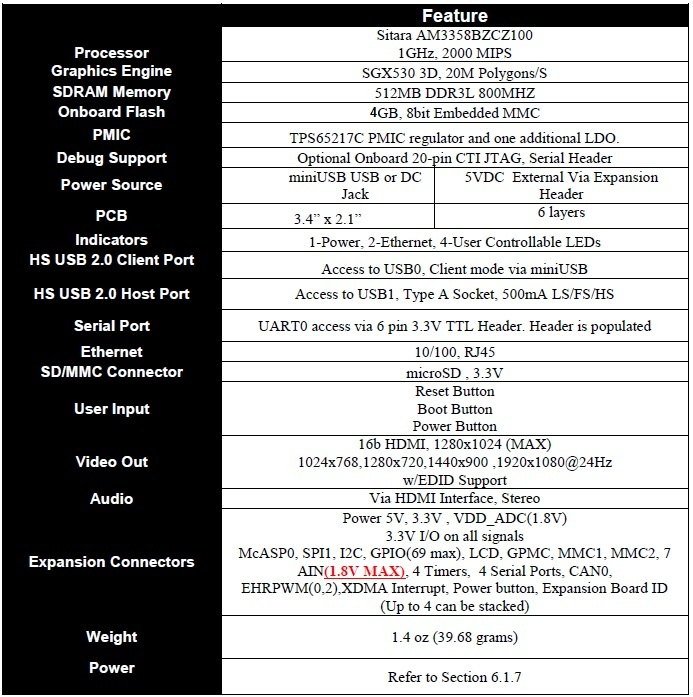
\includegraphics[scale=0.6]{fig/BBB_specs.jpg}
%	\caption{Specification of BBB }
%	\label{fig:bbb_specs}
%\end{figure}

 \begin{table}[h]
 	\caption{BeagleBone Black Specifications}
		\begin{center}
			\setlength\arrayrulewidth{1pt}
			\begin{tabular}{|c|c|}
				\hline
				Processor & Sitara AM3358BZC 1 GHz, 2000MIPS\\ \hline
				SDRAM Mem & 512 MB DDR3L 800MHz \\ \hline
				Onboard Flash & 4GB, 8-bit Embedded MMC \\ \hline
				\multirow{3}{*}{Serial Port(s)} & UART0-4 via 6 pin header 3.3V TTL\\
				 								& HS USB 2.0 Client ports, \\
				 								& USB0 access to client via mini-USB\\
				\hline
				HS USB 2.0 Host Port & Type -A Socket 500mA \\
				\hline
				Ethernet & 10/100, RJ45 \\
				\hline
				SD/MMC Connector & microSD, 3.3 V\\
				\hline
				Video Output & 16b HGMI, 1280x1024 (MAX)\\
				\hline 
				\multirow{4}{*}{Expansion Connectors} & Power 5, 3.3V \& VDD\_ADC (1.8v),\\
														&  GPIO(69 Pins), GPMC,  MMC, \\
														& 7 ADC in-pins, XDMA Interrupt, \\
														& Power button, Expansion Board ID\\
				\hline
				
			\end{tabular}
		\end{center}
\end{table}

As we can see from the specification it is a very capable hardware but the most important feature of this board is the PRU-ICSS, Programmable Real-time Units Industrial Communication Subsystems. Which are two independent 200MHz 32bit RISC processors cores, they operate completely independent from the the ARM core,  allowing independent operation and clocking for greater efficiency and flexibility. The PRU-ICSS enables additional peripheral interfaces and real-time protocols. In addition they have highly predictable latency, they are connected to (almost) all peripherals with Enhanced Data Bus (for GPIO) for better communication. PRUs can be programmed separately by loading them with a binary file. Brief description of PRUs are given below

\subsection{PRU Subsystem}
The Programmable Real-Time Unit Subsystem and Industrial Communication Subsystem (PRU-ICSS) consists of dual 32-bit RISC cores (Programmable Real-Time Units, or PRUs), shared data, and instruction memories, internal peripheral modules, and an interrupt controller (INTC). The programmable nature of the PRU, along with its access to pins, events and all SoC resources, provides flexibility in implementing agile real-time responses, specialized data handling operations, custom peripheral interfaces, and in offloading tasks from the other processor cores of the system-on-chip (SoC).

\begin{figure}
	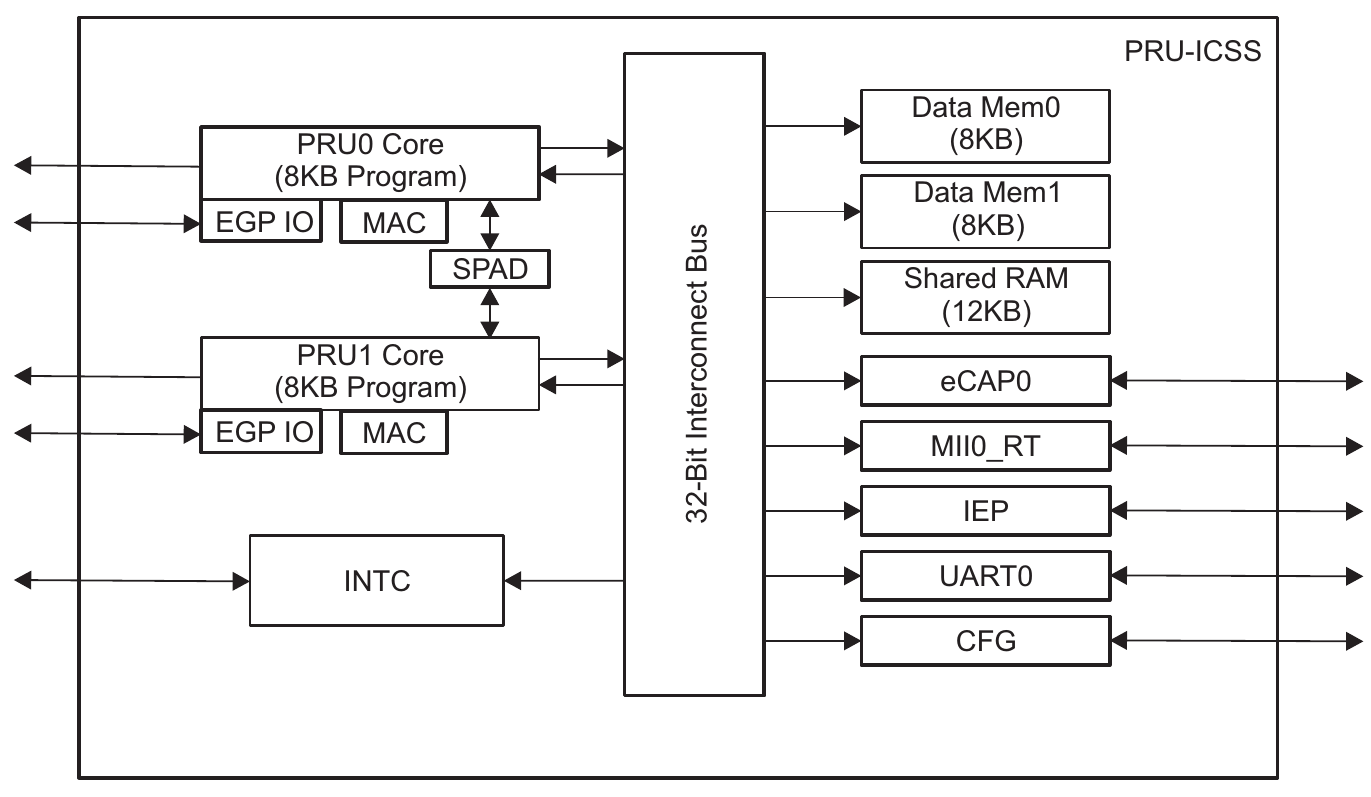
\includegraphics[width=\textwidth]{fig/PRUIcss.png}
	\caption{Block Diagram of PRU Subsystem}
	\label{fig:prublkdrg}
\end{figure}

Useful features that we are using and are worth noting are as follow:
\begin{itemize}
	\item Two PRUs each with:
	\begin{itemize}
		\item 8KB program memory
		\item 8KB data memory
		\item High Performance Interface/OCP Master port for accessing external memories
		\item Enhanced GPIO (EGPIO) with async capture and serial support
		\item Multiplier with optional accumulation (MPY/MAC)		
	\end{itemize}
	\item Scratch pad (SPAD) memory with 3 banks of 30, 32-bit registers 
	\item Broadside direct connect between PRU cores within subsystem
	\item 12 KB general purpose shared memory
	\item One Interrupt Controller
	\item One 16550-compatible UART with a dedicated 192-MHz clock.
\end{itemize} 

\subsection{ADC Subsystem}
AM3358 has 200ksps 8 channel multiplexed single SAR type ADC on it. It is important to understand the functioning of ADC system because we are using few specific features in our implementations (viz Steps, Open Delay and Sample Delay). AM3358 has Touch Screen Controller and Analog to Digital Converter system combined (know as TSC\_ADC\_Subsystem) \cite{AM3358TRM} . Few main feature of ADC Systems are: 
\begin{itemize}
	\item[--] Programmable FSM sequencer that supports 16 steps.
	\item[--] Software register bit for start of conversion
	\item[--] Dual Conversion Modes: One-shot \& Continuous
	\item[--] Sequence through all input channels based on a mask
	\item[--] Programmable OpenDelay before sampling each channel
	\item[--] Programmable sampling delay for each channel
	\item[--] Programmable averaging of input samples - 16/8/4/2/1
	\item[--] Differential or singled ended mode setting for each channel
	\item[--] Store data in either of two FIFO groups
	\item[--] Dynamically enable or disable channel inputs during operation
\end{itemize}
AM3358's ADC system is very flexible and hence bit complicated to use. Each function is controlled by a ``step" so each activated feature (either ADC or TSC) is assigned a step number between 1-15 (step -0 is charge step, for touch screen; Step-16 idle) and accordingly the sequencer will iterate through the steps and there by channel(s). sequencer is completely software controlled so the sampling trigger or delay can be configured programmatically.
\begin{itemize}
	\item \textbf{Open Delay \& Sample Delay:} User can decide when the voltage should be driven to the ADC and when should ADC start sampling. This delay is used for letting the voltage stabilize in case of weak signal input or impedance mismatch.This is \textit{Open Delay}. Sample Delay decides the width of the SoC width.
	\item \textbf{Averaging of Sample:} ADC system has an averaging system which averages 1(no averaging), 2, 6 ,8 12 and 16 times. If averaging is turned ON, say for N samples then ADC system will immediately re-sample the signal (same channel) N times, will average all the samples \textit{and then} will put it to FIFO buffer.
	\item \textbf{Single-Shot or Continuous Mode:} In Oneshot mode sequencer finishes the sampling and conversion of all enabled channels, disables the channels and waits for another trigger. In continuous mode, sequencer loops back to the first step to restart the conversion process all over again, till the STEPENABLE bit is reset.    
\end{itemize} 

\section{Implementation Overview}
An overview of PMU implementation, using AM335x based BeagleBone Black is show in Fig: \ref{fig:implementation}.

\begin{figure}[h]
	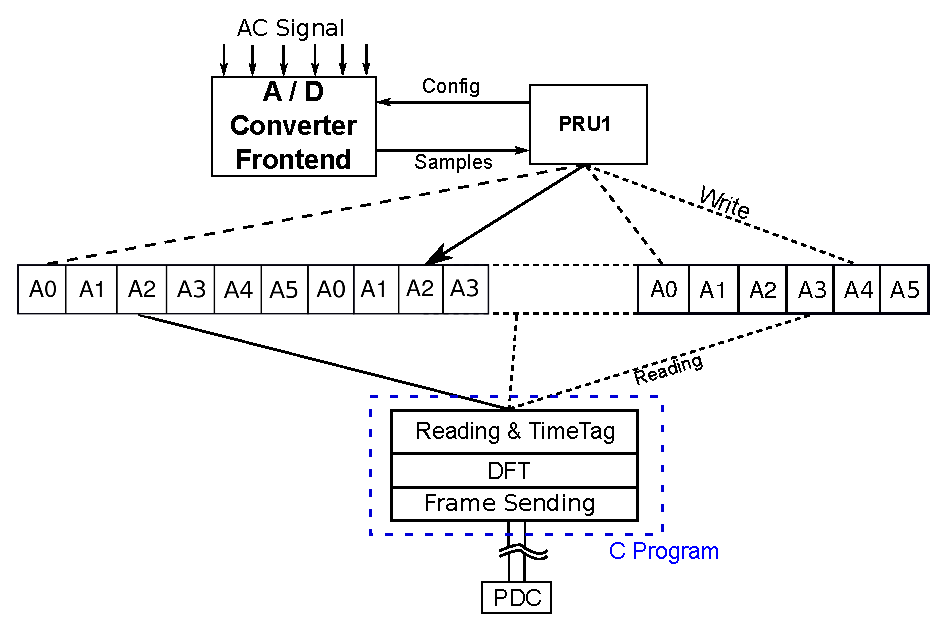
\includegraphics[width=\textwidth]{fig/sys_overview.eps}
	\caption{Overview of implementation}
	\label{fig:implementation}
\end{figure}

The implementation being described is a synchronized operation of three independent asynchronous subsystems: PRU, ADC and ARM core. Overall configuration of system upon which project has been built ,the environment under which programs were developed and ran is, Debian - 7.5 (Wheezy) LTS, running on Linux Kernel version \texttt{3.8.13-bone50 \#1 SMP}. 

\begin{itemize}
	\item ARM side C program is written which programs the PRU and uploads a binary file in to them (PRU1). PRU binary files does three task:
	\begin{enumerate}
		\item Configure ADC, with 
		\begin{itemize}
			\item Enables 6 channels by writing to \texttt{STEPCONFIGx} \footnote{Kindly refer to \cite{AM3358TRM} for further details regarding these registers.}
			\item Configures Open Delay (\texttt{OpD}) = 0, by writing zeros to \texttt{STEPDELAYx} register  
			\item Sample delay (\texttt{SaD}) = 0 
			\item Sample Averaging (\texttt{SAvg}) = 1  by writing ones to  \texttt{STEPCONFIGx} registers
			\item Timer delay [\texttt{Tmr}]= 156250 ns
			\item \texttt{Mode} = continuous 
		\end{itemize}
		\item Define the memory to be used as buffer and size of buffer
		\item Parse the data received from FIFO buffer (of ADC) in to the ring buffer. 
	\end{enumerate}
	\item 6 ADC channels are enabled and the sampling rate is set to 128 samples/cycle/channel (using \texttt{Tmr} delay). the OpenDelay and Sample Delay are kept zero because our signal strength is enough. Timer delay is configured to $ \frac{1}{128 * 50} = 156250 ~ns $.
	\item In continuous mode the buffer is defined as ring buffer and the   buffer length is kept $ 128 * 6 = 768 * 2 = 1536 $. buffer length is kept double for reading and filling the buffer in Ping-Pong fashion.  
	\begin{figure}[h]
		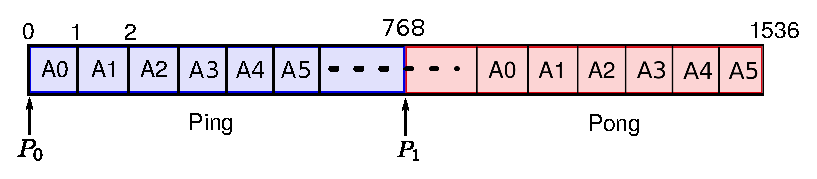
\includegraphics[width=\textwidth]{fig/ring_buffer.eps}
		\caption{Ring Buffer length and Ping Pong depicted}
		\label{fig:rb_pp}
	\end{figure}
	\item C program after uploading the bin file, sets the execution bit. This initiates the PRU execution, which signals ADC to start sampling with given configuration. PRU continuously fetches the the data from the output FIFO register of ADC and puts it in to ring buffer \textit{continuously} and sequentially in ascending order of enabled channels [ \texttt{A0 A1 A2 A3 A4 A5 A0 A1.....A4, A5}].
	\item On the ARM side C program creates two pointers and using Ping Pong method over ring buffer reads the ADC samples in chunks. Brief description of how this works is described below and see Fig: \ref{fig:ping_pong}.
	\begin{itemize}
		\item[--] A buffer of size double then the target size is created (here of 1536 words) and two pointers  \texttt{P0} and \texttt{P1} are created, which points to the start and the middle of the buffer respectively. [ Step - 1 ]
		\item[--] Out of two pointer one works as \texttt{write head} and other as \texttt{read head}. So P0 keeps the track of number of ADC samples parsed in the buffer. [ Step-2 ]
		
		
		\begin{figure}
			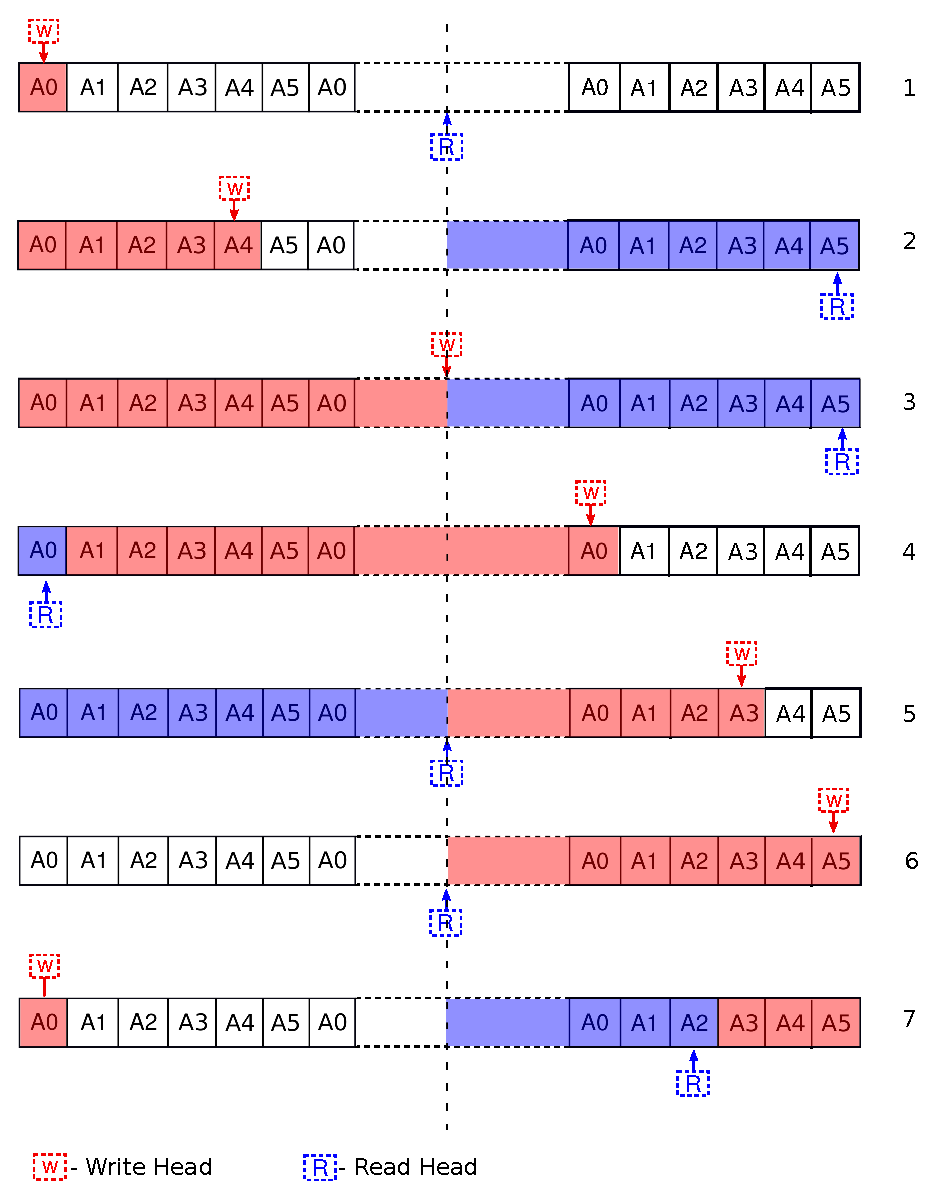
\includegraphics[width=\textwidth]{fig/ping_pong.eps}
			\caption{Ping-Pong Process Visualized}
			\label{fig:ping_pong}
		\end{figure}
		
		
		\item When P0 (write head) reaches 768 samples (128* 6, one whole cycle of all channels), pointers are swapped, P1 becomes the write head and P0 becomes the read head and goes to the beginning of the buffer and starts reading, while write head (pointer P1) continuous to write samples into buffer [ Step-3 ]
		\item Read operation is faster then write ( as PRU has to wait for the samples to arrive depending upon the sampling rate). Read head reaches the middle while P1 is still writing the samples. [ Step-5 ]
		\item After reaching the end of buffer, pointers are again swapped, P1 again becomes the read head and P0 Write head, which starts reading from the middle and the write goes to the beginning of the buffer and starts filling the samples. [ Step-6 ]
		\item From this point it is same as the beginning and the whole cycle repeats. [ Step-7 ]
	\end{itemize} 
	\item This way C program keeps on toggling between two buffers and there by allowing for concurrent reading and writing operation
	\item A visual depiction of the Ping-Pong process described above is show in the Fig: \ref{fig:ping_pong}
\end{itemize}

\begin{figure}[h]
	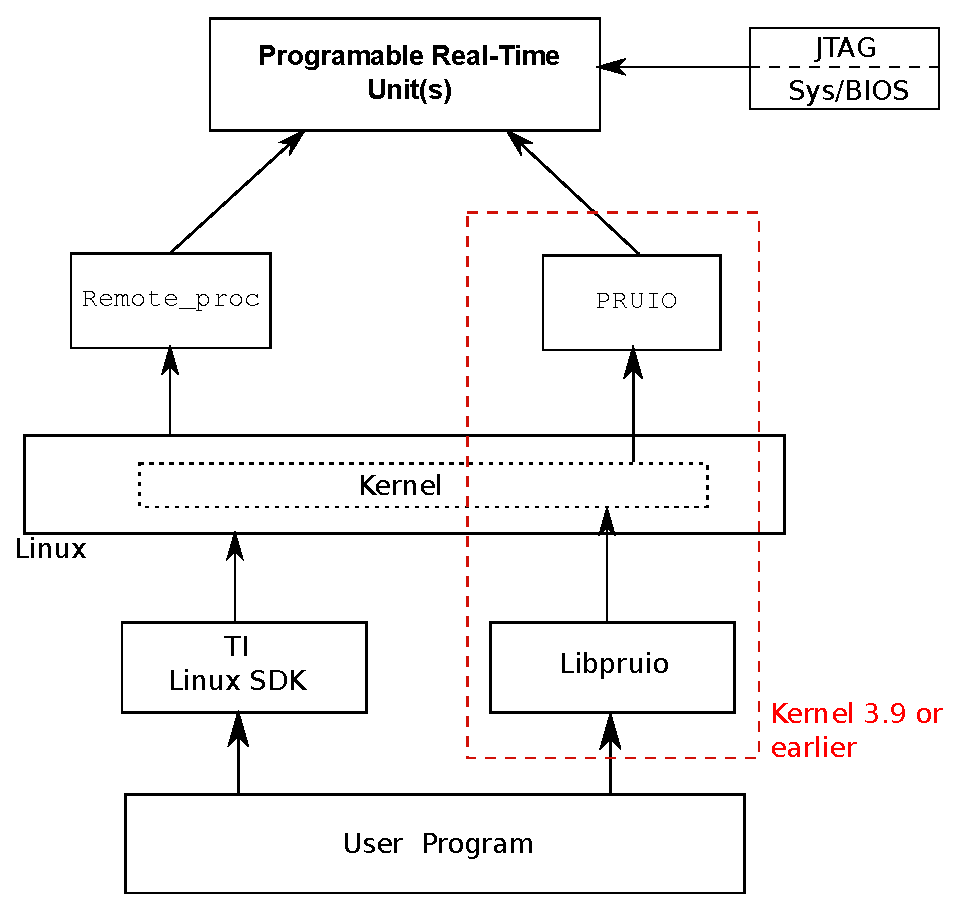
\includegraphics[width=\textwidth]{fig/PRU_config.eps}
	\caption{PRU Configuration Methods}
	\label{fig:pru_config}
\end{figure}

\subsection{PRU Programming}
There are several way to program PRUs, depending upon the kernel version, Operating System and the mode of connection.
\begin{enumerate}
	\item PRUIO - PASM 
	\item Remote\_Proc
	\item Direct firmware loading via JTAG
\end{enumerate}

A visual overview of different way of accessing PRUs is show in Fig: \ref{fig:pru_config}.
\subsubsection{PRUIO}
 For Kernel version older then 3.9 PRUIO kernel module is used which uses a Device Tree Overlay. Device trees are a way to describe Hardware in system, their memory address, their port number or there function. A good example of it would be how UART is described in the system. Device tree enables addition of new hardware in run-time from \texttt{User Space}, in the kernel architecture. 
 
 To go into a little history of why Device Trees (DT) were brought in is that, usually ``Board File" is used in kernel package to describe a hardware of specific embedded system, but given the huge number of ever increasing ARM based devices it was becoming impossible to incorporate all the boards' file in to main Kernel. So Linus Torvalds \cite{DThist} suggested the ARM device developers to use DT, to simplify the kernel maintenance and up-keeping while providing complete flexibility to describe their processor (something that was already being done by PowerPC manufacturers). So, usage of kernel module and Device Tree enables us to configure PRUs and use them. It maps PRU's register memory address to our user space addresses and enables direct access to them. 
 
 A library  called as \textbf{libpruio} \cite{libpruio} is used here, for convenience and rapid development. The library provides C and FreeBasic API's for accessing and configuring ADC, GPIO and PWM modules. It uses converts user C code to Assembly Language via PASM and uploads it to the respective PRUs.
 
 \subsubsection{Remote\_Proc}
 Modern SoCs have multiple processors and processor cores on them in asymmetric multiprocessing (AMP) configuration. which may be running different instances  of operating system, whether it's Linux or any other flavor of real-time OS  . So to enable single kernel to control all those remote processors while abstracting hardware differences and there by reducing the duplication of code \textit{Remote Processor Framework} is used \cite{remoteproc}.
 
 Here in case of AM3358, Remoteproc acts as a framework that allows the ARM host processor(s) to load firmware into PRU cores, start the PRU cores, stop the PRU cores, and configure resources that the PRUs might need during their execution (such as configuring the PRUSS INTC module and providing shared buffers in DDR memory for message passing).

\subsubsection{Direct Loading}
Texas Instruments provides different development mediums for it's products, For  AM335x also, there existed - Sys/BIOS support, TI Starterware support and Ti Processors-SDK support, out of which Sys/BIOS and Starterware are a non-OS solution which posses bare minimum driver support in form of modules, which is very useful in rapid development and due to the absence of OS, latency is brought down to bare minimum.
\begin{figure}[h]
	\centering
	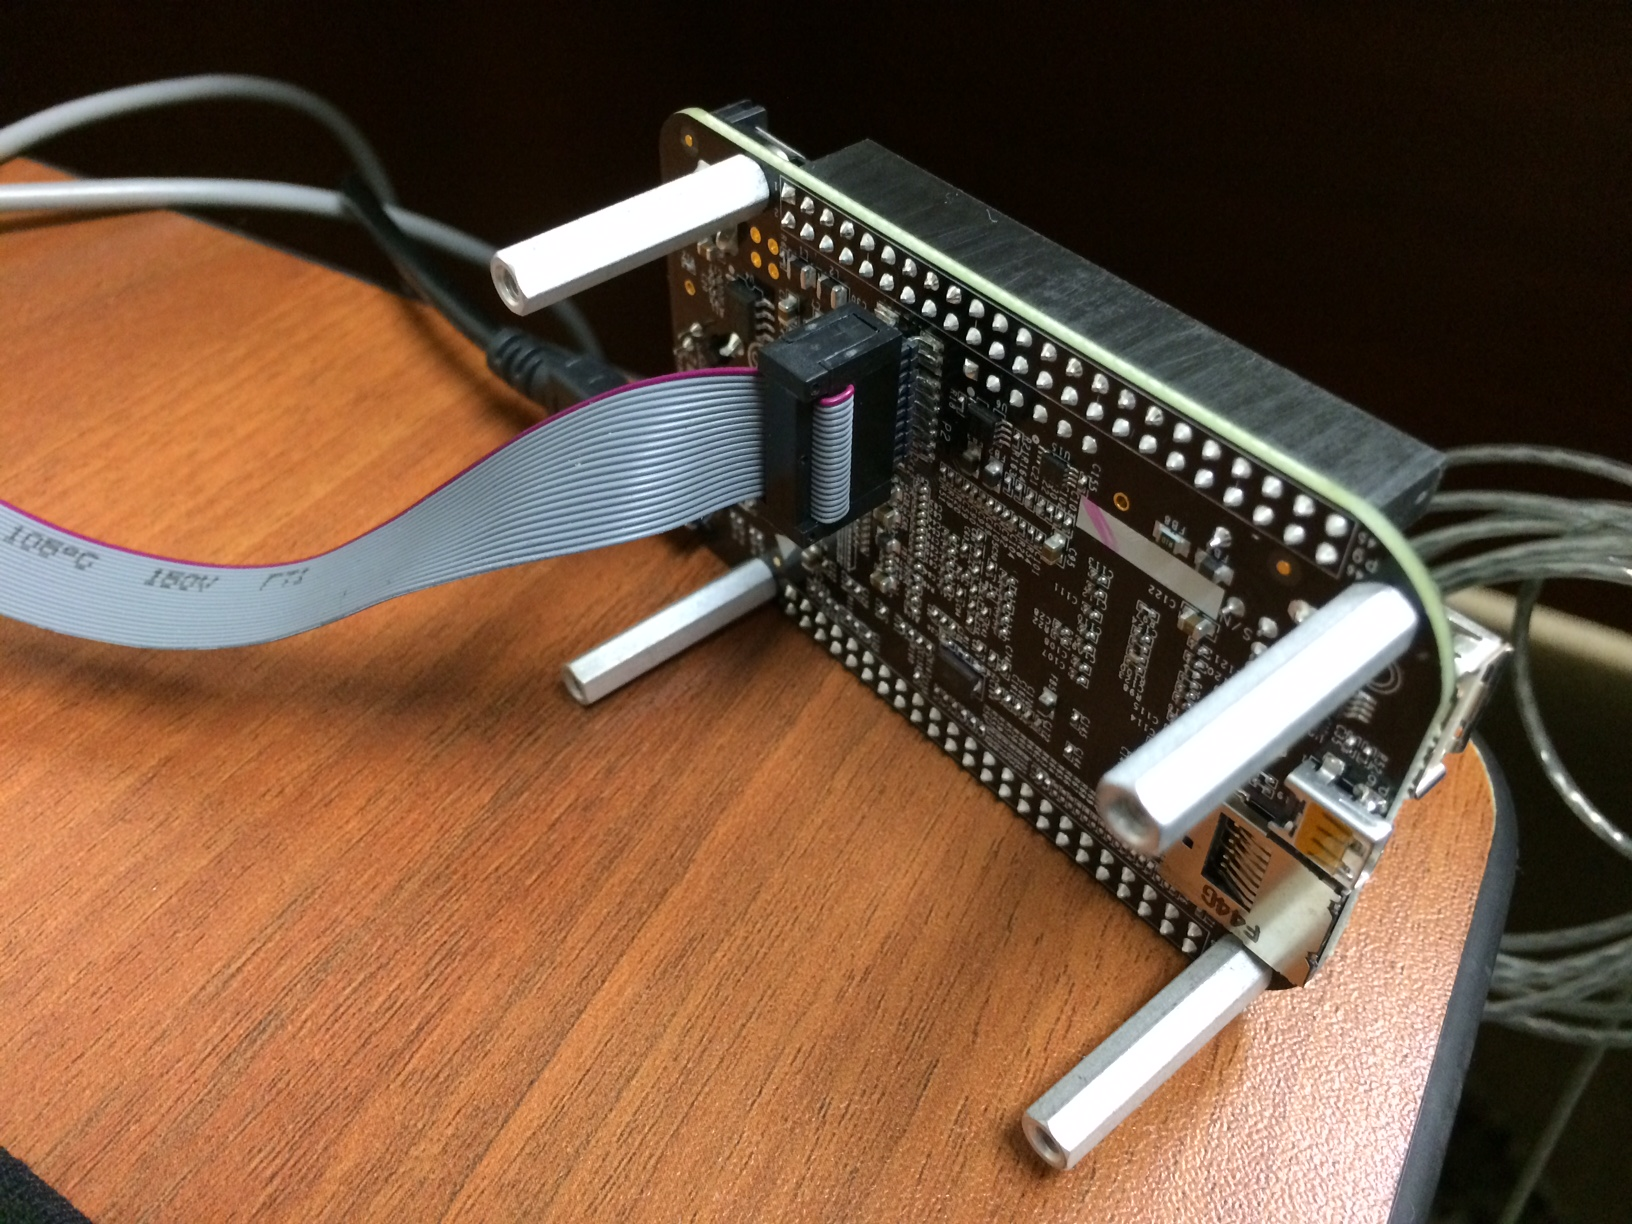
\includegraphics[width=\textwidth/2]{fig/bbb_jtag.jpg}
	\caption{A BeagleBone connected Via Ti's Hawk JTAG}
	\label{fig:BBB JTAG}
\end{figure}

Efforts were made to utilize Sys/BIOS initially for the project but it had become obsolete and was being phased out by Texas Instruments, which resulted into poor support for relatively newer processor like AM3358. Then efforts were made for using TI-Processor SDK as well, but it required a special ARM \texttt{TMDSEMU100v2U-20T} JTAG-extension header-connector (see Fig: \ref{fig:BBB JTAG}) which was not available and hence had to be dismissed. But in principal if one possesses the JTAG, TI-processors SDK can be a very competitive implementation compared to a Linux based implementation, due to real-time capability, direct access to PRU and optimized device drivers by Texas Instruments itself.


\subsection{Time stamp, GPS interfacing and Data Processing }
As seen in the previous section, data is read in chunks each chunk has 768 samples which consists of 128 samples from all the 6 channels. This makes it more convenient to handle and process the data. Using GPS for time reference was aimed but due to hardware interfacing issues, GPS could not be interfaced instead Network Time Protocol (NTP) is being used for time-keeping. Time stamp for each frame is stored on the first sample of the frame written to the buffer.

\begin{itemize}
	\item A moving window type recursive-DFT is implemented. Window length of 2 cycle, 256 samples is chosen for better frequency resolution.
	\item Under the normal operation, each time a sample is removed from the beginning of the window and a new sample is inserted at the end of it. after which a simple DFT is done and which would provide and magnitude and angle of phasors.
	\item Sliding of window is continued for 128 samples (for one whole cycle) after which, the average of all the DFT samples over the whole cycle is done. This result is then sent forward for reporting.
\end{itemize} 

Initially conventional plain DFT was being used, which resulted in to computation time of 1.1 to 1.3 ms, with an error of $\pm 5 \%$ in frequency measurement after which a mixed radix FFT method was tried using a library \cite{kissFFT} which was providing accurate results within range of $\pm1.1\% $ yet the computation time taken by it was of the order of \~11ms, which was unacceptable, after which recursive DFT algorithm was tested, which is giving fairly accurate results with a computation time of the order of 200 to 300 $\mu$s.



\subsection{Communication}

After DFT is calculated we have the necessary information to send. Structure of the frame depends upon the configuration and specification of the PMU. Hence as per standards a configuration frames should be communicated by PMU to PDC, which lists following things:
\begin{enumerate}
	\item Time Format 
	\item Number of phasors
	\item Format of the phasor (rect or polar)
	\item Frequency
	\item Number of digital status, if any
	\item Error Bit
\end{enumerate}

The frame configuration used by our device is as show below:
\begin{itemize}
	\item Device ID
	\item TimeTag 
	\item 6 phasor entity 
	\item Frequency
\end{itemize}

Once the device is turns ON, it waits for the incoming connection from PDC. Once a connection is established PMU still waits for the ``start" command. After a start command is sent PMU starts sending the data to the PDC. Currently PDC is implemented by us, just accepts the data and writes to file rather then parsing in to a database, it receives the data over ethernet via TCP/IP, separates each information from frames and writes it to a file. For evaluation purposes the communication delay, sampling delays and reporting time are computed. This is done by computing the time difference between two frame received, by measuring time difference between two time tags of consecutive data frames and by measuring the time taken for the data packets to be received. 

\subsection{Input Circuit}
BeagleBone Black ADCs are extremely sensitive and operate at very low voltage of +1.8v, hence an interfacing circuit was designed to connect BeagleBone Black to the external world safely. Interfacing circuit was doing three functions (1) Input filtering (2) Voltage scaling (3) Voltage Shifting.

\begin{figure}[h]
	\centering
	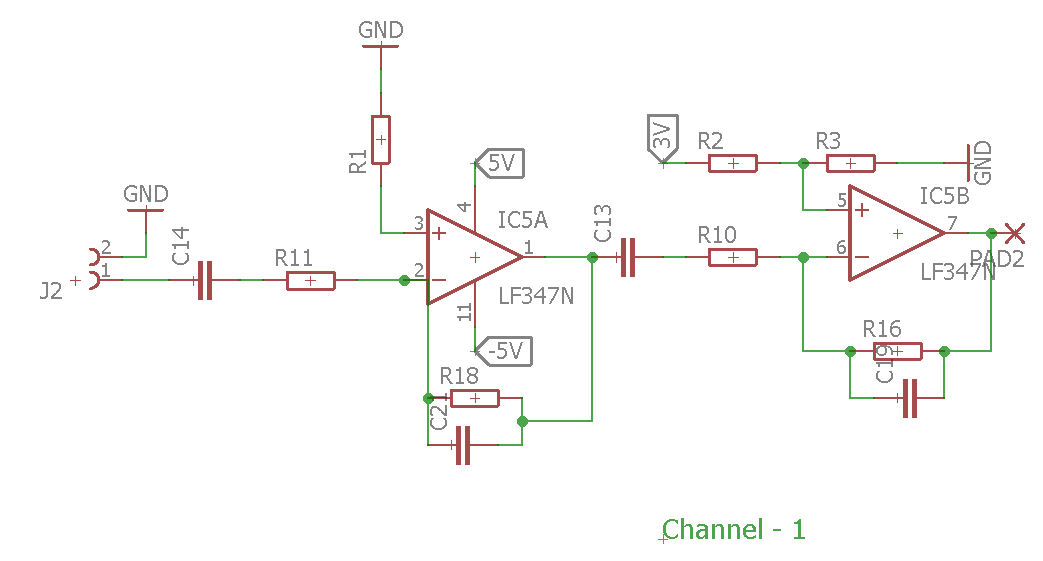
\includegraphics[width=\textwidth]{fig/input_circuit.png}
\end{figure}

Two opamps are used to make two inverted amplifier forming a second order anti-aliasing filter. along with filtering, voltage gain is set such that first stage provides scaling down of voltage for input voltage up $ \pm 20$v and second opamp is provided DC bias on positive input, causing a dc shift in output of the second stage, which brings the output between 0.100 V to 1.6 V which is compatible to ADC input.

\section{Challenges Faced}
There were several challenges faced and solved which are worth mentioning for others who might embark on this path and face it

\begin{itemize}
	\item GPS module interfacing
	
	NavSync CW-12 TIM GPS module is chosen for providing time to the device. The difficulty faced was two fold (i) It was neither getting interfaced with PC nor with BeagleBone Black (ii) It was not locking on to satellites. 
	\begin{itemize}
		\item The second problem of not locking on to satellite got solved. The issue was of insufficient current supplied by the power source.
		\item The second problem of interfacing the module with PC and BeagleBone black is still unsolved. GPS module has serial interface, it is interfaced with PC via USB to serial converter (FTDI RS232L), \texttt{RxD} and \texttt{TxD} , \texttt{GND} pins are connected to FTDI board and \texttt{Vcc} \& \texttt{GND} pins are connected to DC supply of 3.3 V and USB port is connected to PC. This is a standard setup but doesn't function, no data is received from the module. A special utility is provided by Motorola called \textit{WinOnCore} for configuring the GPS module which also fails to connect to the device. To solve this following this were also tried:
		\begin{itemize}
			\item Using a self-made dedicated DC supply instead of standard Regulated DC power supplies devices but to no success.
			\item Connecting the GPS module directly to the BeagleBone Black and powering it from the on-board 3v3 power out. Which also didn't work. Though GPS module was able to lock on to 3 satellites and 1 PPS signal was functional but there is no data being received from the GPS module.
		\end{itemize}   
	\item The situation becomes more challenging to debug when, the device starts sending data when ground connection between transmitter and receiver is made open. the moment ground pin is disconnected GPS module starts sending properly formatted yet, junk data.
	\end{itemize} 
	
	\item DFT computation time:
	
	 
	PMU's DFT requirements are not so complicated and the computational power at hand is also limited, hence plain DFT was implemented but it was taking huge time to compute on ARM processor. Initial latency observed was as high as $4.23 ~ms$/channel. Which was optimized by implementing recursive DFT, along with \texttt{look-up tables}. And another compiler level optimization was done by passing special control flags to the GCC compiler (more details in appendix-B). Now each DFT operation typically takes 340 to 500 $\mu s$/channel. 
	
%	\item Overlapping ADC samples 
	
\end{itemize}